\subsection{Graphing with the Python (Matplotlib library)}

Python is a high-level, interpreted, general-purpose programming language. Its design philosophy emphasizes code readability with the use of significant indentation. Python is dynamically-typed and garbage-collected.
We will use the python language with the language a package called matplotlib. This package is a collection of several plotting libraries. It is endorsed by Matlab but Matlab is paid the stuff i am showing your is free.


\begin{figure}[htb]
\centering

\includegraphics[width=0.15\textwidth]{python.png}
\caption{Python Programming Language Logo}
\label{fig:python}
\end{figure}

\begin{figure}[htb]
\centering
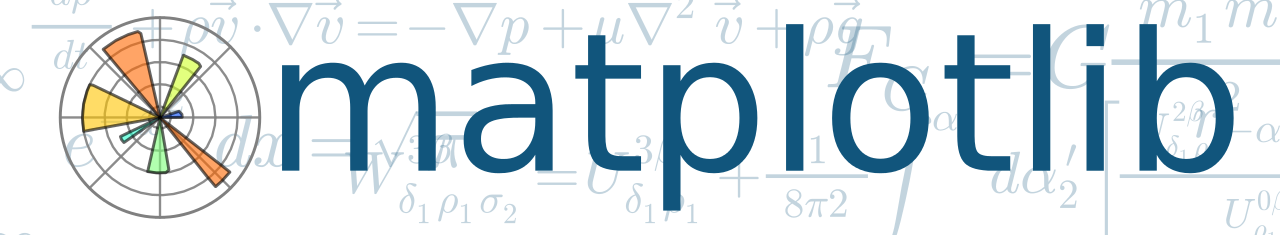
\includegraphics[width=0.25\textwidth]{matplotlib.png}
\caption{Matplotlib Logo}
\label{fig:matplotlib}
\end{figure}
    
\subsubsection{Setting up environment}

First you need to install Python. This is done by opening a terminal and typing the following:
Note this is for linux users.
\begin{lstlisting}[language=bash]
sudo apt-get install python3    
sudo apt-get install python3-pip
\end{lstlisting}

For windows users, you can download the python installer from here: https://www.python.org/downloads/ or install it using the windows store.

Then you need to install the matplotlib package. This is done by typing the following:
\begin{lstlisting}[language=bash]
pip install matplotlib
\end{lstlisting}

pip or pip3 depending on the pip you got ...

If you are struggling check out some tutorials on YouTube on Python or do a course on it.

\subsubsection{Python Demo plotting 3D Graphs}
I have created this demo to showcase some 3D Graph sketching with Python + Matplotlib Library. I wont explain code but consider these examples as a starting point.
Consult the web for library documentation for certain functions being used in my code samples below.

Check out https://matplotlib.org/ for more information on the Matplotlib library.

\begin{lstlisting}[language=Python]
import numpy as np 
import matplotlib.pyplot as plt 
import mpl_toolkits.mplot3d

#plot 3d planes 2x+2y+3z=0 and 3x+5y+7z=0

#increase dpi
plt.rcParams['figure.dpi'] = 200
x = np.linspace(-5,5,100)
y = np.linspace(-5,5,100)
X,Y = np.meshgrid(x,y)
Z = 2*X+2*Y+3
fig = plt.figure()
ax = fig.add_subplot(111, projection='3d')
ax.plot_surface(X,Y,Z,alpha=0.2)
Z = 3*X+5*Y+7
ax.plot_surface(X,Y,Z,alpha=0.2)
### you can add more graphs here ... following this procedure
ax.set_title('2x+2y+3z=0 and 3x+5y+7z=0')
plt.show()
\end{lstlisting}

\begin{figure}[H]
\centering
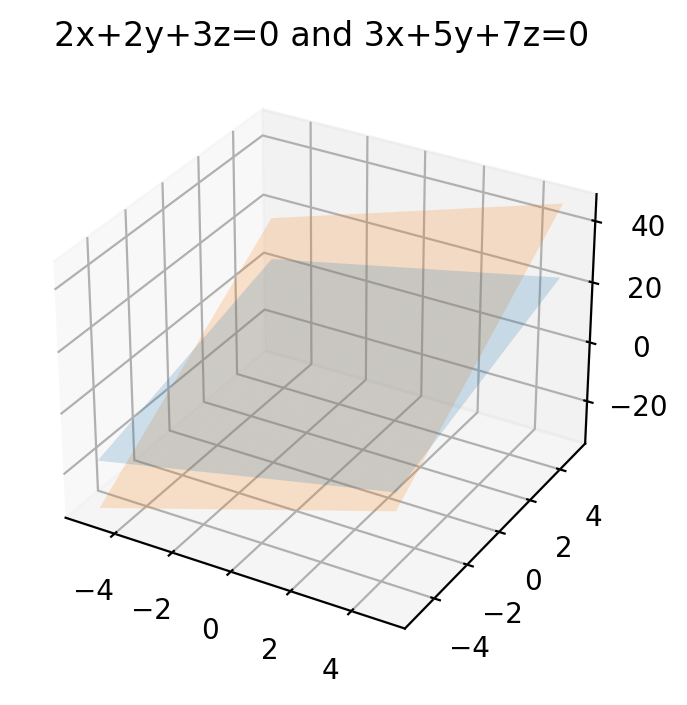
\includegraphics[width=0.5\textwidth]{output_1_0.png}
\caption{3D Graph of $2x+2y+3z=0$ and $3x+5y+7z=0$ generated with Matplotlib}
\label{fig:line3d}
\end{figure}

\begin{lstlisting}[language=Python]
import numpy as np 
import matplotlib.pyplot as plt 
import mpl_toolkits.mplot3d
#increase dpi
plt.rcParams['figure.dpi'] = 200
#plot 1/2*cos(x+y)
x = np.linspace(-5,5,100)
y = np.linspace(-5,5,100)
X,Y = np.meshgrid(x,y)
Z = 0.5*np.cos(X+Y)
fig = plt.figure()
ax = fig.add_subplot(111, projection='3d')
ax.plot_surface(X,Y,Z,alpha=0.2)
#show title
ax.set_title('1/2*cos(x+y)')
plt.show()
\end{lstlisting}    

\begin{figure}[H]
\centering
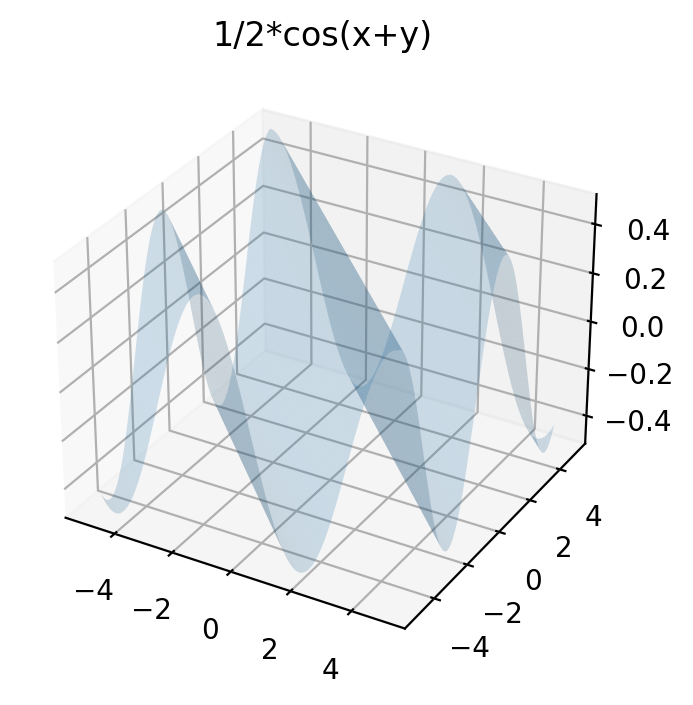
\includegraphics[width=0.5\textwidth]{output_2_0.png}
\caption{3D Graph of $\frac{1}{2}\cos(x+y)$ generated with Matplotlib}
\end{figure}

\begin{lstlisting}[language=Python]
def f(x, y):
    return np.sin(np.sqrt(x ** 2 + y ** 2))
#increase dpi
plt.rcParams['figure.dpi'] = 200
x = np.linspace(-6, 6, 50)
y = np.linspace(-6, 6, 50)
X, Y = np.meshgrid(x, y)
Z = f(X, Y)
fig = plt.figure()
ax = plt.axes(projection='3d')
ax.contour3D(X, Y, Z, 50, cmap='rainbow_r')
ax.set_xlabel('x')
ax.set_ylabel('y')
ax.set_zlabel('z')
#set title of equation
ax.set_title('sin(sqrt(x^2+y^2))')
plt.show()
\end{lstlisting}

\begin{figure}[H]
\centering
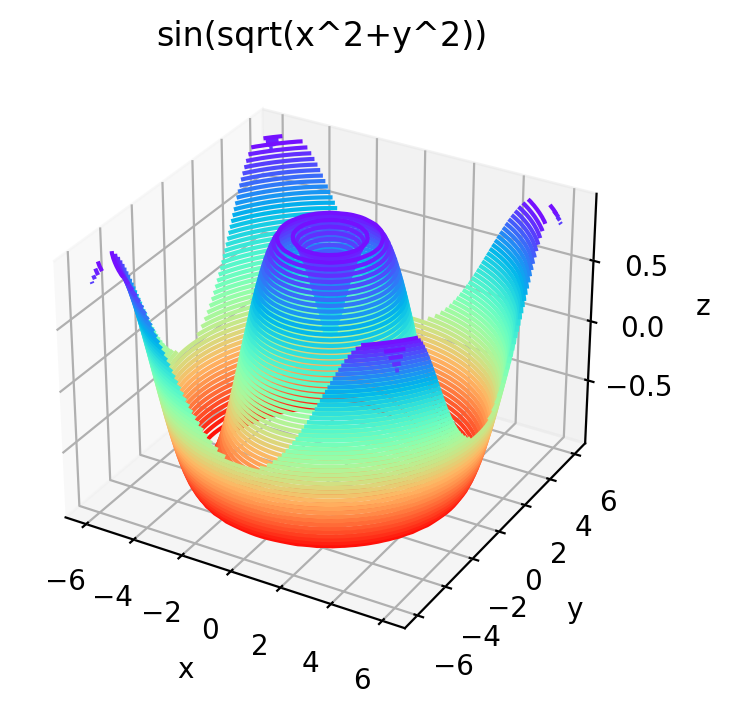
\includegraphics[width=0.5\textwidth]{output_3_0.png}
\caption{3D Graph of $\sin(\sqrt{x^2+y^2})$ generated with Matplotlib}
\end{figure}

\newpage

\begin{lstlisting}[language=Python]
import numpy as np 
import matplotlib.pyplot as plt 
import mpl_toolkits.mplot3d

#increase dpi
plt.rcParams['figure.dpi'] = 200

#plot x^2+2y+5=0 in 3d
x = np.linspace(-5,5,100)
y = np.linspace(-5,5,100)
X,Y = np.meshgrid(x,y)
Z = X**2+2*Y+5
fig = plt.figure()
ax = fig.add_subplot(111, projection='3d')
ax.contour3D(X,Y,Z,50,cmap='twilight_shifted')
#show title
ax.set_title('x^2+2y+5=0')
plt.show()
\end{lstlisting}
\begin{figure}[H]
\centering
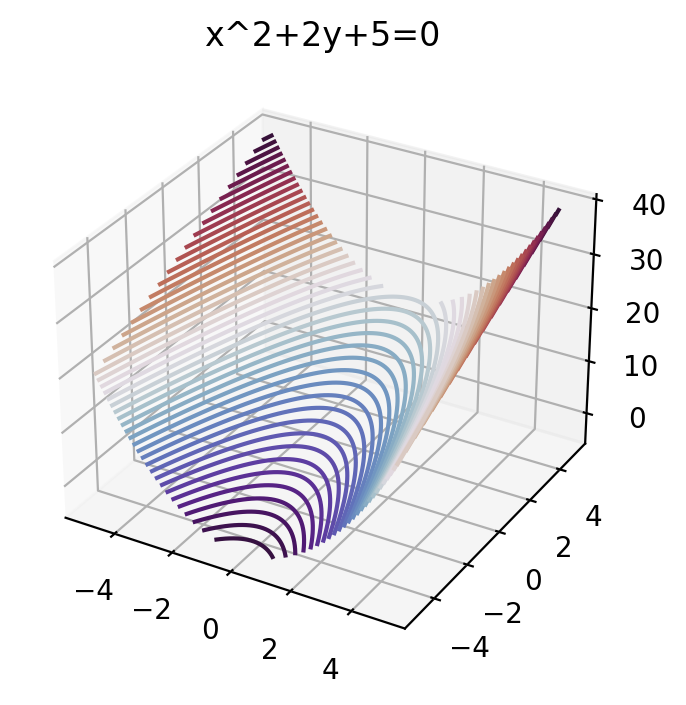
\includegraphics[width=0.5\textwidth]{output_4_0.png}
\caption{3D Graph of $x^2+2y+5=0$ generated with Matplotlib}
\end{figure}

\newpage
From manpulating my code you could easily explore and graph any function you desire. You can be creative with the colors, shapes, and sizes of the graphs.
If you want to just play around have fun! I hope you enjoy my demo and code sample.

This library is so powerful you can do anything possible with it the creativity and research is up to you.




\newpage

\subsection{Graphing with Geogebra (Online Web Platform)}
For the purposes of this paper, we will use the Geogebra Web Platform. This is a free online platform that allows you to graph 3D graphs and equations. You dont need to be logged in to use this platform or install anything on your computer. This is a website/cloud platform.
GeoGebra is an interactive geometry, algebra, statistics and calculus application, intended for learning and teaching mathematics and science from primary school to university level. GeoGebra is available on multiple platforms, with apps for desktops, tablets and web.

%insert figure
\begin{figure}[htb]
\centering
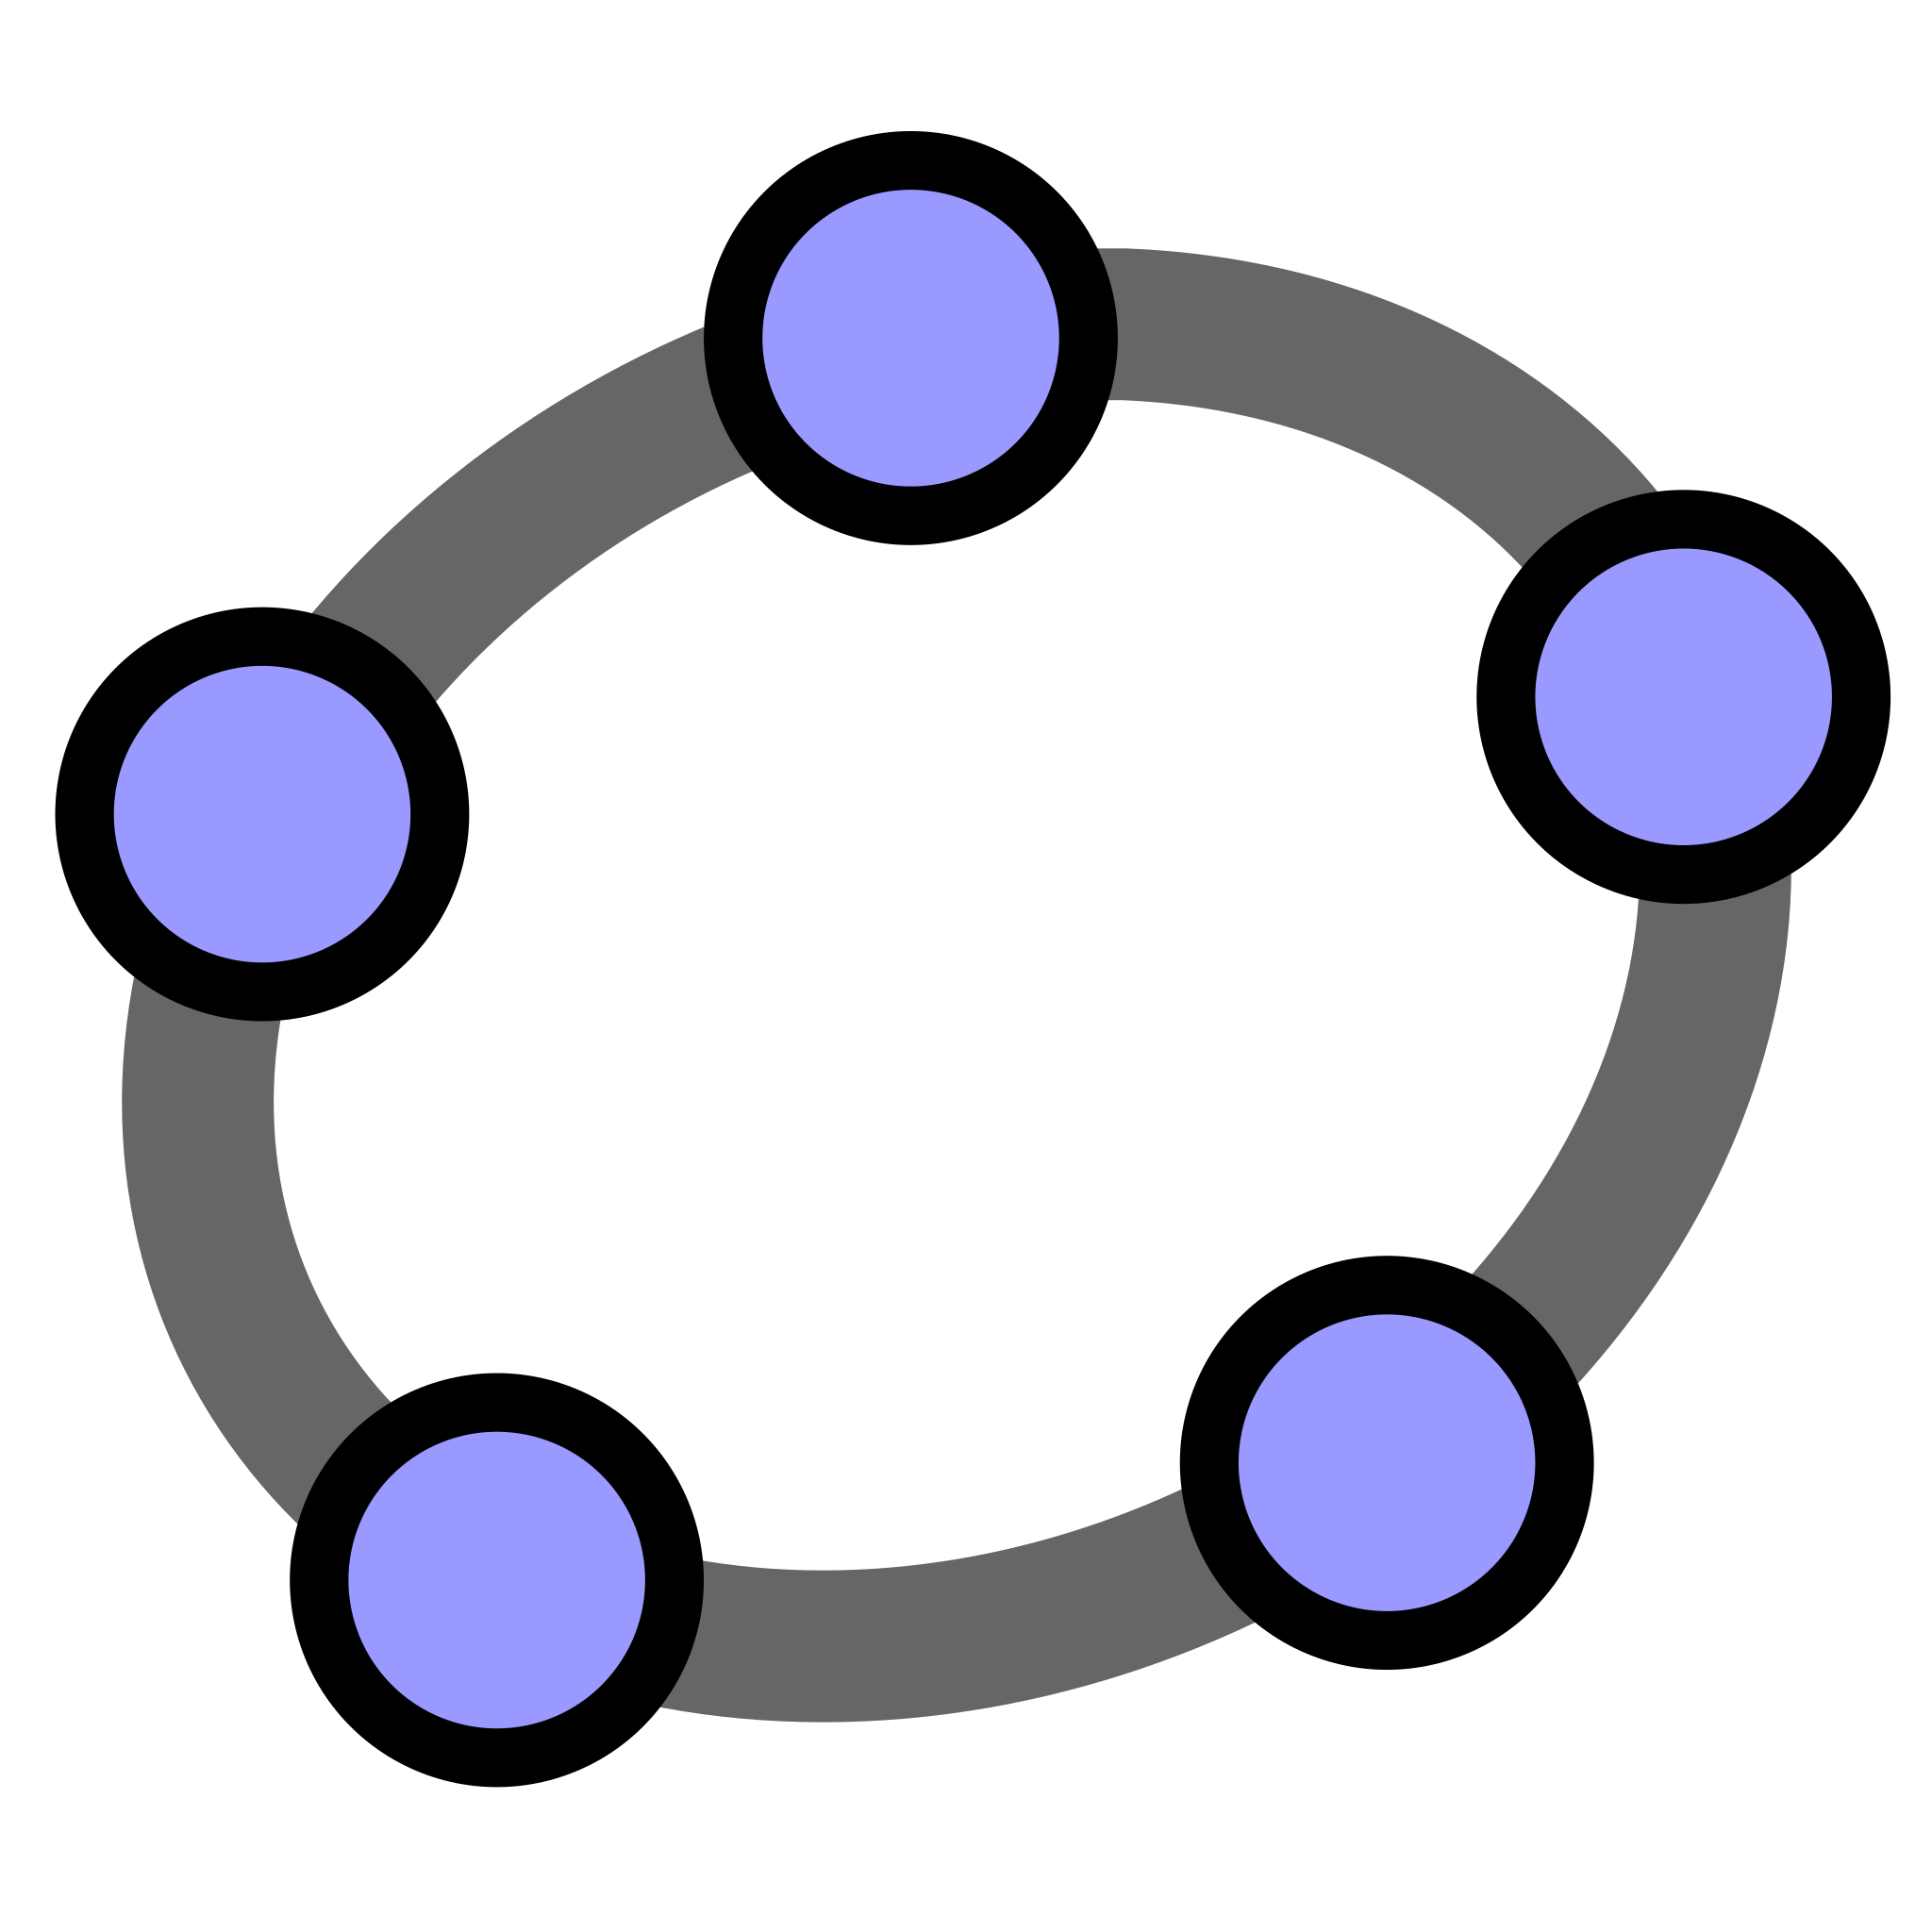
\includegraphics[width=0.4\textwidth]{geogebralogo.png}
\caption{GeoGebra Logo}
\label{fig:geogebra}
\end{figure}



\subsubsection{Our first Geogebra session}

To get started with Geogebra, we will first create a new Geogebra workspace. This is done by opening a new Geogebra window which is followed by going to this link:
https://www.geogebra.org/3d?lang=en

it would look like this below:
\begin{figure}[htb]
\centering
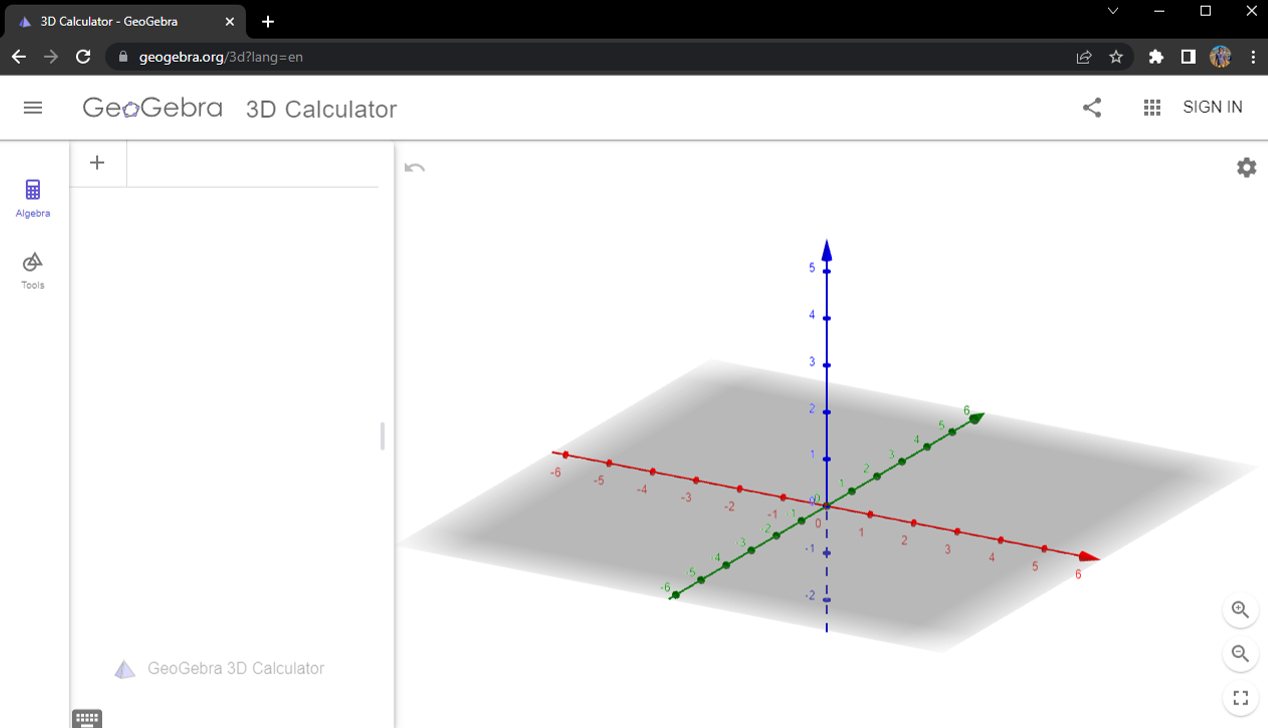
\includegraphics[width=0.9\textwidth]{geogebra.png}
\caption{GeoGebra Workspace}
\label{fig:geogebraworkspace}
\end{figure}

You can now get started with graphing.

For additional things to do check out the tools in the tools tab. It looks like something like this.
\begin{figure}[htb]
\centering
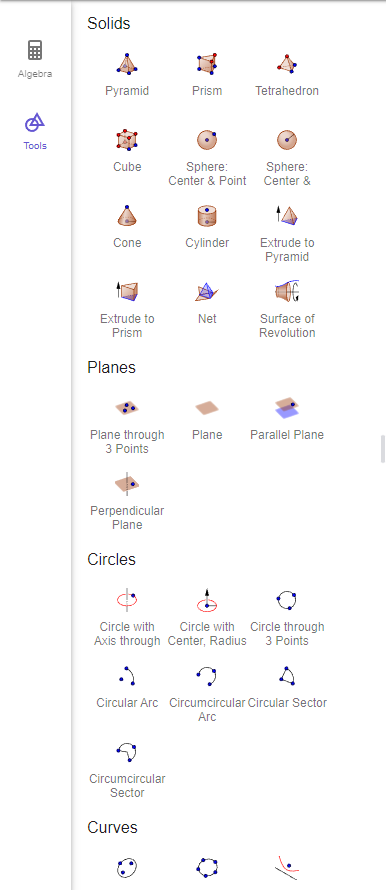
\includegraphics[width=0.4\textwidth]{tools.png}
\caption{GeoGebra Tools}
\label{fig:geogebratools}
\end{figure}

The way you learn is by experimenting have fun!

\newpage

\subsubsection{Plotting equations and vectors}
To plot any equation just type it in the Geogebra workspace. And for plotting a point in the 3D space. Just express your vector as a tuple of coordinates.

In this diagram i have plotted some 3D equations and vectors.

\begin{figure}[htb]
\centering
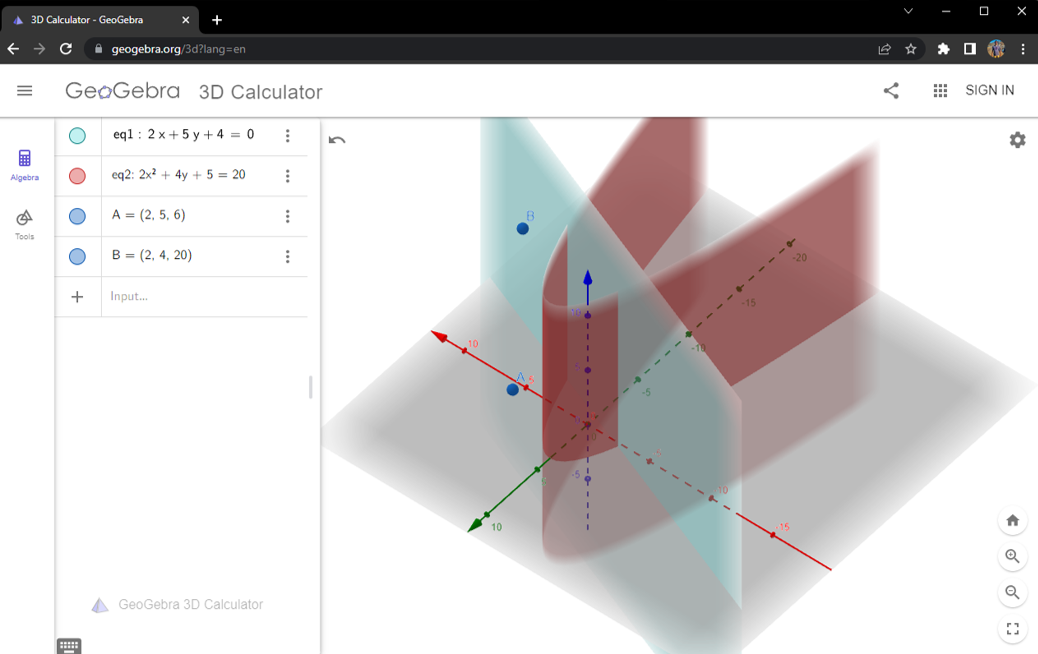
\includegraphics[width=0.8\textwidth]{3d-graph.png}
\caption{GeoGebra Workspace with Equations and Vectors}
\label{fig:geogebragraphs}
\end{figure}

